\documentclass{article}
\usepackage{polski}
\usepackage{listings}
\usepackage{graphicx} % Required for inserting images
\usepackage{xcolor}
\usepackage{float}
\newcommand{\bigO}{\mathcal{O}}

\lstdefinestyle{mystyle}{
    backgroundcolor=\color{white},   % kolor tła
    commentstyle=\color{green},      % kolor komentarzy
    keywordstyle=\color{blue},       % kolor słów kluczowych
    numberstyle=\tiny\color{gray},   % kolor numerów linii
    stringstyle=\color{red},         % kolor ciągów
    basicstyle=\ttfamily\footnotesize, % styl podstawowy
    breakatwhitespace=false,         % łamanie wierszy tylko w białych znakach
    breaklines=true,                 % łamanie długich wierszy
    captionpos=b,                    % pozycja podpisu
    keepspaces=true,                 % zachowanie spacji
    numbers=left,                    % numery linii po lewej stronie
    numbersep=5pt,                   % odstęp numerów linii
    showspaces=false,                % nie pokazuj spacji
    showstringspaces=false,          % nie pokazuj spacji w stringach
    tabsize=2                        % rozmiar tabulacji
}

\renewcommand{\lstlistingname}{} % Usunięcie nazwy "Listing"

\title{Sprawozdanie - Lista 1}
\author{Jakub Zdancewicz}
\date{}

\begin{document}

\maketitle

\tableofcontents
\newpage

\section{Wstęp}
Sortowanie to jeden z fundamentalnych problemów informatyki, mający szerokie zastosowanie w wielu dziedzinach. Algorytmy sortowania odgrywają kluczową rolę w działaniu wielu programów, a ich wydajność istotnie wpływa na szybkość działania. Wybór odpowiedniego algorytmu sortującego jest zatem istotną decyzją podczas tworzenia oprogramowania. W niniejszym sprawozdaniu zajmiemy się analizą trzech algorytmów sortowania:
\begin{itemize}
    \item Insertion Sort
    \item Merge Sort
    \item Heap Sort
\end{itemize}
Wszystkie algorytmy zostały przetestowane na tablicach o tej samej długości, zawierających losowo zainicjalizowane liczby rzeczywiste z zakresu $[-1000000, 1000000]$.

\section{Opis zaimplementowanych algorytmów}
Wszystkie algorytmy zostały przetestowane na 10 tablicach z losowo zainicjalizowanymi elementami dla każdej z 15 wybranych długości. Elementami tablicy są liczby rzeczywiste z zakresu $[-1000000, 1000000]$. Minimalna długość tablicy wynosi 2, a maksymalna 100000. Liczba operacji dla danej długości jest określona wzorem:
\[
    L = \frac{\sum_{n=1}^{10} porownania_i + przypisania_i}{10}
\]
gdzie:
\begin{itemize}
    \item[] $L$ - liczba operacji
    \item[] $porownania_i$ - liczba porównań dla i-tej tablicy
    \item[] $przypisania_i$ - liczba przypisań dla i-tej tablicy
\end{itemize}
\subsection{Insertion Sort}
\textit{Insertion Sort} to algorytm działający w czasie $\bigO(n^2)$. Poniżej przedstawiamy kluczowy fragment jego implementacji:
\newpage
\begin{lstlisting}[style=mystyle, language=C++, caption={Implementacja Insertion Sort}, label={lst:insertion}]
void insertion_sort(float A[], int n)
{
  for (int i = 1; i < n; ++i)
  {
    float x = A[i];
    int j = i - 1;
    while (j > -1 && A[j] > x)
    {
      A[j + 1] = A[j];
      --j;
    }
    A[j + 1] = x;
  }
}
\end{lstlisting}

Algorytm w i-tym kroku pętli \textbf{for} wstawia element $A[i]$ do wcześniej posortowanej części tablicy $A[0] \leq A[1] \leq \cdots \leq A[i-1]$. W pętli \textbf{while} przesuwamy wszystkie elementy większe od $A[i]$ o jeden indeks w prawo, a następnie wstawiamy $A[i]$ na odpowiednią pozycję, czyli po pierwszym elemencie mniejszym od $A[i]$ lub na początku tablicy, jeśli wszystkie elementy są większe.
Poniżej podajemy wynik eksperymentów z tablicami różnych wielkości:
\begin{figure}[H]
    \centering
    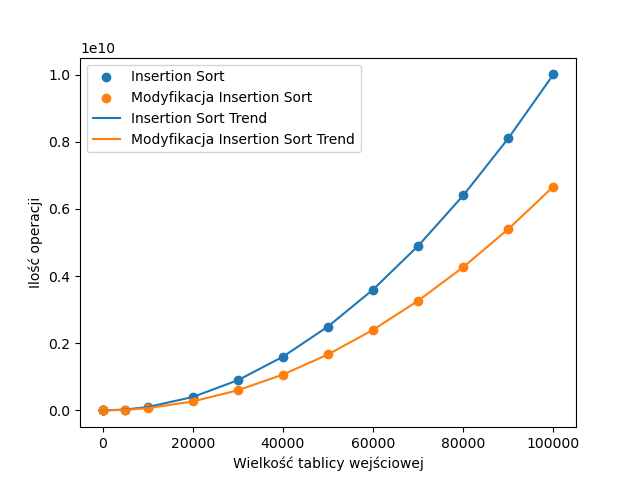
\includegraphics[width=0.8\textwidth]{Figure_1.png}
    \caption{Ilość operacji w zależności od wielkości tablicy wejściowej}
    \label{fig:moj_obraz}
\end{figure}

\end{document}